\documentclass[12pt]{article}

\title{Using idiolects to improve word prediction}
\author{Wessel Stoop}

\usepackage{covington}
\usepackage{graphicx}
\usepackage{float}
\usepackage{apacite}
\usepackage{qtree}

\renewcommand{\familydefault}{\sfdefault}

\usepackage{caption3} % load caption package kernel first
\DeclareCaptionOption{parskip}[]{} % disable "parskip" caption option
\usepackage[footnotesize]{caption}

\linespread{1.5}

\let\stdsection\section
\renewcommand\section{\newpage\stdsection}

\begin{document}

\begin{table}[b]
\begin{tabular}{ll}
\textbf{Master's thesis}&\\
Name&Wessel Stoop\\
Student numbers&s0808709 (Nijmegen), u1249664 (Tilburg)\\
Supervisor&Antal van den Bosch\\
Period&Spring 2013\\
\end{tabular}
\end{table}

\maketitle

\begin{figure}
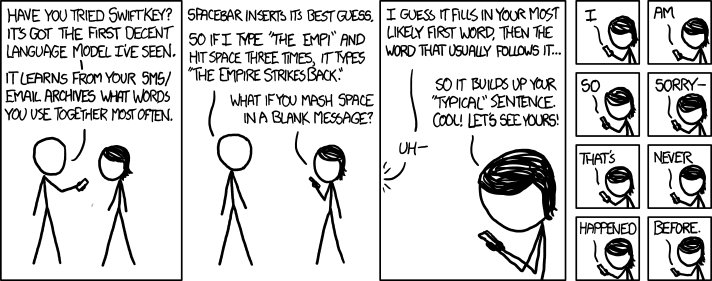
\includegraphics[scale=0.5]{swiftkey}
\end{figure}

\clearpage

\tableofcontents
\listoftables
\listoffigures

\section{Summary/samenvatting}

\subsection{English}

\subsection{Nederlands}








\section{Introduction} \label{intro}

In this thesis, I will show that the concept of \emph{idiolects}, the language of one person, can be used to improve \emph{word prediction}. Because these are two separate topics from the field of Natural Language Processing and the field of sociolinguistics respectively, I will introduce them separately: word prediction will be introduced in \ref{word_prediction}, idiolects in section \ref{idiolects}. Section \ref{linking} will explain how these two can be linked.

\subsection{Word prediction} \label{word_prediction}

\subsubsection{The task}

\textbf{Word prediction}, \textbf{word completion} or \textbf{autocompletion}, is the task of predicting what a user is going to type, as he/she is typing. This can be either the current word, as shown in sentence \ref{current_word}, the next word, as shown in sentence \ref{next_word}, and possibly even more words after that. 
\begin{examples}
\item I'd like some c$|$ookies \label{current_word}
\item I'd like some $|$cookies \label{next_word}
\end{examples}

The text before the vertical bar is what the user has keyed in, the part after the vertical bar is what the word prediction system has suggested. The goal of this thesis is to build a system which can do suggestions exactly like this, as accurately as possible. 

Although the three terms (word prediction, word completion and autocompletion) are often used interchangably, I feel \emph{completion} only captures half of what the system described here can do: it not only completes words (example \ref{current_word}), it also predicts new ones (example \ref{next_word}). Therefore, I will consistently refer to the task as \emph{word prediction}, and to the system as a \emph{word prediction system}. With this, I always mean predicting both current words and next words.

Word prediction is used in many applications we use daily: Google completes our search queries, our webbrowser finishes the web addresses we type in, our email client finishes email addresses, Excel completes annotations based on earlier annotations, etc. It reduces the number of keystrokes we have to do, and thus saves us time and effort. However, when we type full sentences, whether they are part of an email, a scientific article, a tweet, or a master's thesis, we often still key in every single character. 

Why don't we use word prediction here too? While no quantitative research has been done to answer this question, an obvious answer would be that prediction accuracy generally is too low to speed up typing. Keying in every character is often faster than checking and accepting the predictions. Once typing speed decreases, however, word prediction \emph{is} used. With the rise of smartphones,  on which one  cannot type as fast as on a normal keyboard, word prediction has become more widely known - although it is unclear what proportion of the smartphone users also use some sort of word prediction application. Another example are  people with speech and motor disabilities, like cerebral palsy or hemiplexia. By using a device equiped with word prediction technology, they can increase their communication rate considerably \cite{Garay-Vitoria+06}.

\subsubsection{Word frequency as chance indicator}

In the academic literature, several attempts have been done to improve word prediction technology, so that it can increase the communication rate for smartphone users, people with physical disabilities and typing in general. One of the first techniques to achieve a useable word prediction system is to use frequency lists; although it is possible to wait until a word unicity point has been reached, much more keystrokes can be saved if the prediction can be done earlier. For example, if the user wants to type the word \emph{communication}, the system could wait until \emph{communicatio} has been keyed in to make sure not do an incorrect suggestion in case the user wanted to say \emph{communicative}, but it could also take the risk and guess one of the words much earlier. 

Which one of the two (\emph{communication} or \emph{communicative}) the system guesses should be the option that is more likely. This chance of occurence of a word is reflected by its frequency in texts: the more a word occurred in the past, the more likely it is to occur again in the future. In the example, \emph{communication} will be more likely to be correct because it will probably be higher on a frequency list. One of the first word prediction systems using this technique, and also one of the first word predictions systems in general, was PAL \cite{swiffin+85}. 

\subsubsection{Context-sensitivity}

Since then, numerous authors have shown that taking context into account improves prediction accuracy significantly \cite[among others]{Lesher+99,Garay-Vitoria+06,Tanaka-Ishii07,vandenbosch+08}. This entails that the system has some information on which words are likely to follow each other, and uses this when giving predictions. For example, if the user has keyed in sentence \ref{iate}, a context-sensitive system should not predict the word \emph{communication}, even if it is high on the frequency lists, because \emph{communication} is unlikely to follow \emph{ate}.

\begin{examples}
\item I ate co \label{iate}
\end{examples}

One of the earliest implementations of this concept by \citeA{hunnicutt87} used a 2D-matrix to store frequent collocations of words. Table \ref{matrix} shows how a matrix based on the training material in \ref{training} could look:

\begin{examples}

\item 

\begin{itemize} \label{training}
\item[(a)] I like dancing.
\item[(b)] You like fishing.
\item[(c)] I ate cookies.
\item[(d)] You ate cake.
\end{itemize}

\item \begin{tabular}{l|ll}
&I&you\\
\hline
like&dancing&fishing\\
ate&cookies&cake\\
\end{tabular} \label{matrix}

\end{examples}

Thus, when this system is offered a new context, like \emph{You like}, it can look this up in the matrix. On the basis of the matrix (and thus indirectly on the basis of the training material), it will predict \emph{fishing} for this context. With this technique, frequency only plays a secondary role: it no longer is important how often a word occurs in general, but how often it occurs in a particular context. So even if we have a training corpus of billions of words in which the word \emph{fishing} is very infrequent, as long as it is the most frequent word in a particular context, \emph{fishing} will be the word predicted when that context is encountered.

Obviously, the accuracy of a context-sensitive system largely depends on how often a similar context was available in the training material; since an algorithm can only know what will follow a particular context if it has seen that context before, we should try to give it as much training material as possible. A key publication by \citeA{Lesher+99} indeed shows that the accuracy of a context-sensitive word prediction system is related to how much training material is provided. Their algorithm can save 46\% of the keystrokes when using 100.000 words (when showing the user the top 10 of most likely predictions), and this percentage slowly but steadily increases when they add more training material: for 200.000 words, it can save 47\%, for 300.000, it can save 48\%, etc.

This does not mean that our ultimate goal is to collect every context possible, however. Not only would this be almost impossible (a language with 10.000 words already has 10.000$^3$ possible trigram contexts), it is also not necessary: most possible trigram contexts are not possible for a language (for example, the 'possible context' \emph{the a of} is ungrammatical, so will probably never occur), and even most possible trigram contexts that \emph{are} grammatical will rarely occur. This has to do with a characteristic of language called \emph{Zipf's law} \cite{zipf65}, named after the American linguist George Kingsley Zipf. It entails that the frequency of any word in a particular text (or in language in general) is inversely proportional to its rank on a frequency list for that text; that is, a very small group of words is used all the time, and a very large group of words are rarely used. For example, according to Wikipedia\footnote{\url{http://en.wikipedia.org/wiki/Zipf's\_law}} in the Brown Corpus for Present-Day American English the most frequent word \emph{the} already covers 7\% of all the material, and the 135 most frequent words of the corpus together cover over 50\% of the material. Similarly, \citeA{lestrade10} shows that for Melville's \emph{Moby Dick}, the plot of the logarithm of the word frequency data (how often a word occurs)  against the logarithm of their rank (position on the frequency list) 'almost follows a straight line': 

%Plaatje moby dick

Again, we see that a few words are used a lot, while most are used only once or twice.

What holds for individual words must also hold, at least to a certain extent, for combinations of words: some combinations are much more frequent than others. Because these combinations are also more likely to end up in the training material, even with relatively few training material a context-sensitive system will perform much better than one would expect on the basis of pure chance. On the other hand, once most of the frequent combinations are covered, it takes more and more training material to improve the results just a little bit. This means we also expect a loglinear distribution for the effect of the amount of training material on the results of a word prediction system. \citeA{vandenbosch11} shows this is indeed the case: in his system, the step from 100 to 900 words in the training material, roughly 6\% more keystrokes could saved (from 15\% to 20\% keystrokes saved), whereas the same is true for the step from 1000.000 to 10.000.000 words (from 40\% to 46\%).

A fact both \shortciteA{Lesher+99} and \shortciteA{vandenbosch11} note is that it is not possible to save 100\% of the keystrokes by simply going on doubling the amount of training material; at a certain point adding more training material does not seem to help anymore. \shortciteA{Lesher+99} hypothize that where that boundary lies depends on how much context the algorithm uses: when more words from the context are used, much more combinations are possible, and thus more training material can be useful. In a hypothetical language with 10 words, 10 contexts are possible when using 1 word as the context, but $10*10*10 = 1000$ contexts are possible when using 3 words as the context. Thus, the larger the context the word prediction system uses, the more contexts are possible, and thus the more the system benefits from having a lot of training material.

As a practical side-note, when using millions of words and all possible combinations between them, and also more context than just two words, a matrix as the one in \ref{matrix} quickly becomes impractical. Modern word predictions systems search through the training material and collect a number of similar contexts. The word that follows most of these contexts will be the word predicted. So when a new context like \emph{You like} is given to such a system, instead of looking it up in a matrix, it compares it to all contexts in the training material. An exact will be found in the sentence \emph{You like fishing}, and thus \emph{fishing} will be predicted. Because comparing a new context to thousands of contexts in the training material might take too much time to do real-time predictions, these comparisons can also be done beforehand, which reduces the process to a decision tree \shortcite[among others]{daelemans+97, vandenbosch+08, vandenbosch11}. The system that will be described in this thesis also uses this technique. See chapter \ref{algorithm} for a detailed description of the algorithm.

\subsubsection{Adding more knowledge} \label{more_knowledge}

Context-sensitivity, in particular when using a lot of training material, is most powerful when it comes to collocations (for example, \emph{in combination with}, \emph{on the basis of}), i.e. when it comes to language. However, humans use more than knowledge of language alone to predict what somebody is going to say; we also take into account what the speaker typically says, and what the speaker is talking about. For instance, the input \emph{wed} can be very likely to refer to \emph{Wednesday} when making an appointment for next week, whereas it can also be very likely to refer to \emph{wedding} when talking about a marriage. In other words, besides the linguistic context, we also want to give the system some 'real world' context.

One way to give some of this kind of knowledge to word prediction systems is to use training material from the same domain; \shortciteA{verberne+12} show that trying to predict Wikipedia text, tweets, transcriptions of conversational speech and Frequently Asked Questions all worked best when using texts from the same type (i.e. training on Wikipedia text to predict Wikipedia text). Furthermore, they show that questions about neurological issues, for which little training material was available, could best be predicted with the corpus that was closest in terms of topics discussed: the medical pages from Wikipedia. 

\citeA{vandenbosch11} takes a completely different approach and tries to make a word prediction system learn about register and topic on the fly with a \emph{recency buffer}. This buffer stores the $n$ latest words; if a word the user is keying in matches one of the words in the recency buffer, this word is suggested instead of what the system would actually have suggested. The idea behind this is that if the user is writing about, for example, traveling, words like 'go', 'hotel', and 'see  will always be in the buffer and thus be suggested. In other words, the systems learns about the user and the topic on the fly.

Although both approaches help to increase the number of keystrokes saved, they also have downsides: for the system by \citeA{verberne+12} training texts in the same genre are needed, which might not be available, whereas the system by \citeA{vandenbosch11} ignores context information that it should weigh more intelligently. For example, while a context-sensitive text-prediction system will probably be able to predict \emph{to} for the sentence \emph{Tommy was going t...}, the one with the recency buffer will predict \emph{Tommy}.


\subsection{Idiolects} \label{idiolects}

\subsubsection{The concept}
Almost every claim done in the field of linguistics concerns language as a whole; whether the subject of investigation is a particular syntactic construction, phonological variable, or some other linguistic phenomenon, the results are always supposed to hold for an entire language variety. The concept of an idiolect, the language of only one person, is well-known, but rarely ever mentioned \cite{mollin09, barlow10, louwerse04}. According to \citeA{mollin09} it is a 'neglected area in corpus linguistics', and \citeA{barlow10} states that the term 'is distinguished by the fact that there is probably no other linguistic term in which there is such a large gap between the familiarity of the concept and lack of empirical data on the phenomenon.' This is remarkable, since 'idiolects are the only kind of language we can collect data on', as \citeA{Haugen72} points out; a language variety essentially is nothing more than a collection of idiolects.

Part of the lack of research in this area can of course be explained by practical limitations (it is hard to collect a lot of data for one person, let alone doing this for multiple persons), but theoretical views have also played a role: for decades, generativism has been the leading linguistic framework. Generativism focuses on \emph{langue} rather than \emph{parole}, and views deviations in actual usage as uninteresting exceptions to an otherwise perfect abstract system. This view was mainly shared by sociolinguists at the time; as \citeA{labov89} puts it: 'language is not a property of the individual, but of the community. Any description of a language must take the speech community as its object if it is to do justice to elegance and regularity of linguistic structure'. However, \citeA{carden70}, himself a generative linguist, points out: 'differences among idiolects have long been an embarrassment for transformational grammarians'.

\subsubsection{Empirical evidence}
Now that usage-based theories of language become increasingly more accepted, and the progress in technology and in particular the internet has facilitated collecting, storing and working with large amount of data, these objections to studying idiolects slowly vanish. One of the first publications investigating idiolects quantitatively is that of \citeA{mollin09}. She created a corpus of speech by the former Prime Minister of the United Kingdom Tony Blair, and compared this to the British National Corpus. Focussing on maximisers ('absolutely', 'totally') and the adjectives, verbs and adverbs they cooccur with, she has compiled a list of collocations that are used much more by Blair than by the general language community. \citeA{barlow10} investigated speech patterns of five White House Press Secretaries, using transcripts of spoken language available on the internet and dividing them in samples of 200.000 words. He compared the frequencies of bigrams and trigrams (like \emph{of the}, \emph{that we} and \emph{and that's}) and discovered that there are significant differences between individual speakers. Interestingly, however, when frequencies from one sample were compared to frequencies from another sample by the same speaker, they were very consistent. For example, Ari Fleischer rarely uses the bigram \emph{we are} in sample 1, and this is also the case for samples 2, 3 and 4, while the opposite is the true for Scott McClellan. To make sure these differences cannot be attributed to lexical preferences, Barlow repeated his research with POS $n$-grams ([article, noun], [preposition, verb], etc) and grammatical constructions ('\emph{noun} of the \emph{noun}',  'will' vs 'going to', usage of the passive, etc.), and shows similar results.

\subsubsection{Practical use}
The reality of idiolects cannot only be seen through the efforts of corpus linguists, however. \citeA{Coulthard04} gives a number of anecdotes where the notion of idiolects have been helpful in court. The most clear example is the story of the so-called 'Unabomber'. This person sent various hand-made bombs to \textbf{un}iversities and \textbf{a}irports (hence the nickname) from 1978 to 1995, killing 3 persons and injuring 23. In 1995, he offered six major newspapers to stop his attacks if they would publish a manuscript he had written, entitled \emph{Industrial Society and its future}. The Washington Post decided to do so. Three months later, a man contacted the FBI, claiming the language looked very similar to the language of his brother, a mathematician called Ted Kaczynski. He had recognized in particular the phrase 'cool-headed logician' to be part of his brother's idiolect. In the cabin where Kaczynski was living at the moment, indeed a wealth of bomb components were discovered, and FBI researchers determined that other texts that were found there could only have been written by the same person. Kaczynski was sentenced to life in prison with no possibility of parole. 

This example shows the concept of idiolect might be more than just an abstract concept used by linguists. It cannot only only be tested empirically, but is actually something the layman can understand and even recognize. Furthermore, this example shows the concept of idiolect might actually robust enough for practical applications.

\subsection{Using idiolects for word prediction} \label{linking}
As was explained at the end of section \ref{more_knowledge}, both the approach of \citeA{vandenbosch11} the approach \shortciteA{verberne+12} of adding more knowledge to the word prediction systems have downsides: the system by \citeauthor{vandenbosch11} uses information that easily available, but cannot be used in a context-sensitive way, and the system by \shortciteauthor{verberne+12} is context-sensitive, but uses information which might not be easily available. In this thesis, a word prediction system based around the concept of idiolects will be built: a system that tries to predict what the user is going to write \emph{on the basis of his  or her own language}. The idea behind is that there is a much higher chance that a system will be able to correctly predict what somebody is going to write if it can look at things this same person has produced earlier, instead of things somebody else using the same language has produced earlier. These idiolect data (1) are more likely to be easily available (for example, by using emails, papers, blogposts, tweets or messages by that same author) and (2) are can be processed beforehand, and thus can be used in a context-sensitive system. In other words, the best parts of both approaches will be combined.

\subsection{The rest of this thesis} \label{restofthisthesis}
As was explained in detail in section \ref{word_prediction}, word prediction systems work with an algorithm and a language model. Language models are formed out of training material, which simply is a large collection of 'example language' - I used the sentences in \ref{training} to illustrate this. To built an as good as possible word prediction system, it is essential to make both the algorithm and the language model as good as possible, so this is exactly what I will do in the rest of this thesis: chapter \ref{algorithm} is about the algorithm, chapter \ref{model} is about the language model, and the thesis will be concluded in chapter \ref{conclusion}. In chapter \ref{algorithm} I will start with a very simple algorithm, and then slowly makes it more complicated. After each addition, little experiments will show to what extent it improves the system. In chapter \ref{model}, various models are compared to eachother, to get an idea of which model will work the best for which situation. 





\section{The algorithm: Soothsayer} \label{algorithm}

\subsection{Introduction}

\subsubsection{Soothsayer} \label{ss_intro}
The goal of this chapter is to build the best word prediction algorithm possible, from the ground up. We will start with a very basic application that uses word uniqueness thresholds to predict the word the user is keying in, and add more components and smaller improvements step by step. I have given the resulting system the working title \emph{Soothsayer}, for ease of reference.

An important thing to note is that Soothsayer works with independent modules. A module can be seen as a function that takes some input (for example, the letters of the word the user is currently keying in) and uses a language model to generate:

\begin{enumerate}
\item The most likely prediction
\item The second most likely prediction
\item The third most likely prediction
\item In case of a context-sensitive module, how many other predictions the model provided
\end{enumerate}

Modules can be either context-insensitive or context-sensitive, as will be explained in much detail in section \ref{ci} and section \ref{cs} respectively, and use one language model. In a set-up with two language models we thus have four possible modules:

\begin{table}[h]
\begin{tabular}{lll} 
Module&Type&Model\\
\hline
1&Context-sensitive&model 1\\
2&Context-insensitive&model 1\\
3&Context-sensitive&model 2\\
4&Context-insensitive&model 2\\
\end{tabular} 
\caption{A possible module set-up}
\end{table}

Modules can be concatenated in such a way that a second module takes over once the first modules no longer has predictions, a third module takes over once the second one no longer has predictions, etcetera. This makes it possible to use multiple prediction techniques \emph{and} multiple language models in one prediction system.

\subsubsection{Evaluation}
In this chapter, I will propose an addition to Soothsayer and then measure to what extent it improves the number of keystrokes saved several times. But how does one measure how many keystrokes are saved exactly? In other words, what is the best way to evaluate a word prediction system?

One possibility is to provide the user with a list of the $n$ most likely predictions \cite{Lesher+99,Fazly+03}. This approach has the advantage that it results in high percentages of keystrokes saved (in particular when $n$ is set to a high value, because this means the system can do multiple guesses at once, while only one has to be correct), but also has downsides. As \citeA{vandenbosch11} notes: 

\begin{quotation}
[I]n many devices and circumstances it is inefficient or impossible to present [...] suggestion lists. Inspecting a list of suggestions also poses a larger cognitive load than checking a single suggestion, and furthermore it is unclear how scrolling, browsing and selecting items from this list should be counted in terms of keystrokes.
\end{quotation}

For this reason, I will follow \citeA{vandenbosch11} and always calculate the number of keystrokes that could have been saved when the user was presented only one prediction at a time. Predictions can be accepted with the space key. Because this is sometimes problematic (for instance, if the user wanted to type \emph{sun}, but Soothsayer predicts \emph{sunday}, hitting space would lead to the wrong word), a rejection is also calculated as a keystroke. The number of keystrokes that can be saved if the autocompletion application works this way will be called \textbf{Classical Keystrokes Saved} (CKS) in the remainder of this thesis.

On the other hand, current popular smartphone applications suggest this approach might be too strict. The popular smartphone application SwiftKey\footnote{\url{http://www.swiftkey.net/}} always shows the user three predictions, which seem to be (1) what the user has keyed in so far, (2) the most likely prediction and (3) the second most likely prediction. In case the user has not yet started typing the next word, option (1) is replaced by the third most likely prediction. Because smartphones use a touchscreen as an input device, no extra keystrokes are needed. The percentage of keystrokes that can be saved when two (and sometimes three) predictions were shown will be referred to as \textbf{SwiftKey Keystrokes Saved} (SKKS).

A thing to notice is that both measures reflect the percentage of keystrokes saved in an ideal situation; that is, when the user accepts a correct prediction immediately once it is available. As will be discussed further in section \ref{early}, this is not necessarily the case. 

%referenties nalezen, meer toevoegen
%wordt dat echt discussed? NEE
%Hit ratio. Time-saving, person saving.

\subsubsection{What Soothsayer is not}
There are many possible approaches to take when building an autocompletion system. Because it would take too much time to try all of these approaches (and all combinations of them), I had to set limitations. Therefore, before I explain and defend the workings of Soothsayer, I therefore would like to list the most importat decisions, so the reader has a rough idea of what is coming. 

\begin{itemize}
\item \textbf{Soothsayer does not predict more than one word at a time}. Some scholars have investigated the possibility to predict multiple words at the same time [[refs]]. This can very fruitful: if a word prediction system knows that \emph{on the b} should be \emph{on the basis of} it makes more sense to offer this as a whole, instead of first asking whether \emph{basis} is correct. However, multiword prediction comes with a lot of downsides: every extra word that is predicted doubles the chance of making an incorrect prediction, it is unclear what a user should do if he/she accepts the first word, but the not the second word (or vice versa), and how this should be counted in terms of keystrokes, and giving multiple words forces the user to plan ahead a few words while typing, which might not be how the user prefers to write. %kijken wat antal zegt

\item \textbf{Soothsayer does not focus on one specific domain of word prediction, but works for word prediction is general}. Niet Google.

\item \textbf{Soothsayer is not designed for mobile phones, but can be integrated into any kind of software, on any device}. When discussing this subject with others, I noted that word prediction is often confused with T9. T9 is a system in which every number corresponds with 3 or 4 characters (\emph{1} = \emph{.,!}, \emph{2} = \emph{abc}, \emph{3} = \emph{def}, etc.). A T9 system allows the users to press all numbers only once, and tries to figure out which word the writer probably intended; for example, \emph{233} can correspond to \emph{bed}. Although there is some language technology involved in systems like these (the system should know enough about language to figure out \emph{aef}, \emph{cfe} \emph{bde}, etc. or not words), this is not what Soothsayer does; Soothsayer does try to guess what the user wanted to say \emph{after} the user keyed it in, but \emph{before}. 

Besides that, Soothsayer is designed to be indepent of device of input method. Instead, it includes a \emph{server mode} and an \emph{HTTP-server mode}, making it very easy to integrate into any piece of software. This means it is very well possible that Soothsayer will be used together with a T9-system one day.

\item \textbf{Soothsayer does not use hand-made, language-specific rules, but is fully language independent}. In the early of Natural Language Processing, many scholars have tried to build NLP systems by including as much as linguistic knowledge of possible. In terms of a word prediction system, this could for example entail including a system that recognizes personal pronouns, and only provides verbs that agree with these pronouns, or making sure that after the neutral article \emph{het} only neuter words were suggested. 

Soothsayer does not work this way. Instead, it is given as much training material as possible, and tries to learn from that. So Soothsayer might know the noun \emph{kast} probably does not follow the article \emph{het}, but because it has not encountered that during training, not because I told it so. As a result of this, Soothsayer is fully language independent: if it is trained on Dutch data, is will predict Dutch words, if it is trained on Swahili, it will predict Swahili words. In fact, the context-sensitive modules will often give correct predictions even with mixed training data.

\end{itemize}

\subsection{Context-insensitive modules} \label{ci}

Context-insensitive modules only use information of the word the user is currently keying in. In sentence \ref{only_c}, for example, only the c will be used for prediction. 

\begin{examples}
\item I ate too much c \label{only_c}
\end{examples}

This means that a prediction like \emph{communication} is fully possible, despite the context, just because \emph{communication} starts with a c. This also means that at the beginning of a each new word no prediction will be available, because the module has no material to work with.

Despite these limitations, context-insensitive modules can already save a lot of keystrokes, because the first few letters of a word impose enormous limitations on what letters can possibly follow.

\begin{examples}
\item This is good communic \label{communic}
\end{examples}

In sentence \ref{communic}, we already know from \emph{communic} that \emph{ation} or \emph{ative} will follow, simply because these are the only two words that start with \emph{communic}. The first iteration of the context-insensitive module I will propose will be based on this idea: at a certain point in a word, other words are no longer an option. This point is called the \emph{uniqueness threshold}.

\subsubsection{First iteration: using uniqueness thresholds}

The first iteration of the context-insensitive module will take the word the user is currently keying in as the input. If, on the basis of what has been given, only one word is still possible, this word will be returned as a prediction. To know which words are 'possible', the module uses a lexicon. An important characteristic of this approach is that is does not or rarely make mistakes (assuming a large enough lexicon): only words the system is 100\% sure about are predicted.

To test this, I exported all emails I have sent between February 2009 and February 2013, containing [[x]] words. I formed a lexicon on the basis of the first 90\% of the material, and tested on the remaining 10\% - the most recent emails. The testing was done by simulating a user keying in the material letter by letter. Once the correct prediction was available, the remaining letters of that word were skipped. The percentages were calculated by dividing the amount of skipped letters by the total amount of letters.

This resulted in a \textbf{CKS of 5\%} and an \textbf{SKKS of 5\%}. These are relatively low percentages, but that can be explained by the fact that many of the words are too short to reach their uniqueness thresholds. For example, the word \emph{the} will never be predicted because even when the word is finished, alternatives are still possible (\emph{these}, \emph{there}, etc.).

\subsubsection{Second iteration: using word frequencies}
A solution to the fact that short words never reach their uniqueness threshold can be to give the prediction \emph{before} the word has reached its recency threshold. This can lead to situations where the correct word is predicted long before the uniqueness threshold is reached, which increases the number of keystrokes saved. However, this also means many incorrect predictions will be given; we sacrifice the accuracy of the system. To what extent this is a problem is unclear: at the one hand, the user is forced to accept and reject more predictions while typing, which probably increases the cognitive load, at the other hand all the user has to do to reject a prediction is to continue typing; no extra actions are needed. A systematic investigation of the extra cognitive load during typing while using a word prediction system is beyond the scope of this thesis; because no extra actions are needed to reject the prediction it will be assumed the saved keystrokes are worth the extra cognitive load.

If a prediction is given when multiple words are still a possibility, a system that picks the word with the highest chance of occurring will of course have the best results. These chances are reflected by the frequency of the words in the language. Therefore, each time the users keys in a new letter, Soothsayer will go through a frequency list. The first (and thus most frequent and most likely) word that matches with what has been keyed in so far will be given as a prediction.

To test this, the email corpus from the previous section was used. The simulation showed a much higher percentage of keystrokes can be saved this way: a \textbf{CKS of 20 \%} and an \textbf{SKKS of 27 \%}. For this reason, this second iteration of the algorithm is the algorithm that will be used when referring to the 'context-insensitive' module in the remainder of this thesis.

\subsection{Context-sensitive modules} \label{cs}

Context-sensitive modules make use of the words that came before the current word to limit what words are predicted. For sentence \ref{only_c}, repeated here as \ref{only_c_r}, the context would be the words \emph{ate}, \emph{too} and \emph{much}.

\begin{examples}
\item I ate too much c \label{only_c_r}
\end{examples}

This context is compared with a training corpus, which results in a list of words which often occur together with the words from the context. This approach probably returns words like \emph{cookies} or \emph{cake} (because of the word \emph{ate}), while the word \emph{communication} is no longer an option because it probably did not occur in this context in the training texts.

\subsubsection{Word prediction as a classification task}

To make use of the context, Soothsayer approaches word prediction as a classification task. Classification means finding a \emph{class} for an \emph{instance} on the basis of its \emph{features}. For instance, you could say a person (instance) is a man (class) because he has a beard, a low voice, short hair and is tall (features). In some cases, classification is simple: when sorting garbage, you use only 1 feature (material) which results in the correct class (paper, glass, plastic, biodegradable, miscellaneous) 100\% of the time, but in most cases it is not; for instance, for a person with a beard you can be pretty sure it is a man, but not all men have beards. And for the other features, there also are women with low voices, women with short hair and women who are tall. In cases like this, it is the combination of features that (in most cases) will result in the correct class.

For word prediction, we use the context as instance, the words in the context as features, and the word which follows this context as class. This means that instead of only two classes (as in the gender example), we have a separate class for every word that could possibly be predicted. Thus, if we want to predict that \emph{cookies} follows the context \emph{ate too much}, we hope that classifying the instance \emph{ate too much} on the basis of its features (the words \emph{ate}, \emph{too} or \emph{much}) will result in the correct class label \emph{cookies}.

\subsubsection{Nearest neighbour classification}

There are many algorithms to do classification automatically. Soothsayer uses the $k$-nearest neighbour classification method. $k$-nearest neighbour classification (henceforth \emph{KNN}) means that the class is determined on the basis of similar cases in a training corpus. How many cases are taken into consideration, $k$, can be determined beforehand. For example, let us set $k$ to 1 and take the following instances as a training corpus:

\begin{examples}
\item one two three (four)
\item one two and (three)
\item one two plus (four)
\end{examples}

The first three words are the instances, the fourth word (between parentheses) is used as the class label. If we then classify a new instance \emph{one two three}, a KNN algorithm will look at these training instances, and decide whether they are similar enough to taken into consideration. What exactly is taken as the definition of 'similar' differs per algorithm; we will follow the IB1-algorithm \cite{aha+91} and simply count how many features overlap. The instance \emph{one two three} is extremely similar: three of the three features match. We then look at the class of this similar example (four), and give this as a result. Simply said, in this case the context-sensitive module will predict \emph{four} because it had exactly the same context in its training corpus, and that context was followed by \emph{four}.

If we set $k$ to 2, both \emph{one two and} and \emph{one two plus} become a possibility as well: they both have two matching features. If we count instances with the same amount of matching features as 1, we now end up with three similar cases. Because most of these cases have \emph{four} as a class label, four will be predicted. Note that \emph{nearest distance classification} would actually be a better name for what we are doing here: we do not use the $k$ nearest neighbours, but \emph{all} nearest neighbours from the $k$ nearest distances [[ref tibml]].

Because the many class labels used for word prediction, Soothsayer always uses a $k$ of 1.

\subsubsection{IGTree}

An important thing to notice from the three training instances in the example is that the third feature is the only feature that has relationship with the class label. The first two features are always \emph{one} and \emph{two} respectively, regardless of the class, and thus cannot be used to find out to which class this instance belongs. This is what is used in the in the IB1-IG algorithm, an variation on the IB1 algorithm mentioned previously: because they have a better relation to the class label, some features are given more weight in the decision process.

This idea that some features can be more useful than others can even be used on a much deeper level to solve another problem: the IB1 algorithm generally is too slow to be used in practical applications, like Soothsayer. While the classification in the example above can be done in a split second, this is not the case for word prediction based on a lot of training material: a training corpus of ten thousand words means that a new instance has to be compared to ten thousand training instances for every character the user keys in. This takes too long, even for powerful computers, and is not necessary. This can be best explained with an example. Let us take the following four instances as our training corpus:

\begin{examples}
\item I ate those (cookies)
\item I ate that (cake)
\item I saw those (zebras)
\item I saw that (elephant)
\end{examples}

Whereas the first feature again has no relation with the class, the second one clearly has: as soon as we see \emph{ate}, we know that the classes \emph{zebras} and \emph{elephant} are no longer an option, and that it is of no use to 'keep them in mind' as an option.

This is exactly how the IGTree algorithm \cite{daelemans+97} works: it calculates which features contain most information about the class labels, and orders the features from most information to least information. It then goes through these features one by one, and at each point 'throws away' the training instances which are no longer an option. This reduces classification to making a small number of decisions (in our case 3, because we have 3 features), instead of comparing thousands of strings. A possible decision tree for the training instances above can be seen in \ref{igtreetree}.

\qtreeshowframes 

\begin{examples}
\item \Tree [.{\emph{ate} or \emph{saw}?} [.{ate: \emph{those} or \emph{that}?} {those: cookies} {that: cake} ] [.{saw: \emph{those} or \emph{that}?} {those: zebras} {that: elephant} ]] 

\label{igtreetree}
\end{examples}

But what happens if we ask IGTree to classify \emph{I ate these}? At the second node, \emph{these} is not one of the features, so the algorithm cannot make a decision. If a classification gets 'stuck' somewhere, which is almost always the case because the users can of course type anything they want, Soothsayer asks the algorithm to return everything which was still a possibility at that point; the classes \emph{cookies} and \emph{cake} in our example. For each possible class, \emph{confidence values} can then be calculated. Confidence values correspond to the percentage of all instances still possible that had that class. The result for \emph{I ate these} in our example would thus be \emph{cookies} with a confidence value of 0.5 (1 of the 2 instances still possible had this class), and \emph{cake} with a confidence value of 0.5 (1 of the 2 instances still possible had this class). %confidence checken

In practice, what Soothsayer's context-sensitive modules do is:

\begin{enumerate}
\item Starting \emph{timblserver}, a software suite of Memory-based Learning software, which includes IGTree (ref). Timblserver is similar TiMBL, but get its input using socket communication. This allows Soothsayer to keep the program running, instead of reloading the tree into memory every single time a classification is needed.
\item Every time the user keys in a character, collecting the last three words, and sending them to the Timblserver.
\item Collecting the output, and picking the word that matches with what already has been typed so far. If more words match, pick the one with the highest confidence.
\item Returning this word as a suggestion.
\end{enumerate}

%socket communication?

\subsubsection{The experiment}

To investigate how many keystrokes can be saved when using context information, as described in the previous paragraphs, an experiment very similar to the experiment for the context-insensitive modules was carried out: a training corpus was created on the basis of 90\% of all of the emails I sent between February 2009 and February 2013, and the results were tested on the remaining 10\%. The percentage were calculated by dividing the amount of skipped letters by the total amount of letters. This resulted in a \textbf{CKS of 24\%} and an \textbf{SKKS of 27\%}.

\subsection{Other decisions}

\subsubsection{Concatenating context-sensitive and context-insensitive modules} \label{concat}
In the previous two sections, we saw that the context-insensitive had a CKS of 20 \% and an SKKS of 27\%, whereas the context-sensitive one had a CKS of 24\% and an SKKS 27\%. This means that using a context-sensitive module over an context-intensive only gives us an improvement of 4\% for the CKS and no improvement for the SKKS, while it is much more complicated and computationally expensive. Is using context-sensitive modules worth that?

The answer, as I will show, is yes. The context-sensitive module learns about which words in the training texts typically follow eachother, and thus is powerful when it comes to the more frequent, fixed combinations of words and words that often occur in eachother's context, but fails when it comes to words that are also frequent, but were not used earlier int his context. The context-insensitive module, on the other hand, can predict any word, as long as it has been used before, but knows nothing about fixed combinations. In other words, one module succeeds where the other fails, and vice versa; there is very little overlap in the situations in which they both do the correct prediction. 

This means that it would make sense to concenate context-sensitive and context-insensitive modules, but in which order? Should the context-insensitive module take over when the context-insensitive module no longer has suggestions, or the other way around? Based on the fact that the context-sensitive module alone performs a bit better, it is likely that the results will be slightly better when the context-sensitive module is tried first. Two simulations, one which each of the orderings, confirmed this, as shown in table \ref{results_concat}.

\begin{table}[h]
\begin{tabular}{l|ll} 
&CKS&SKKS\\
\hline
Context-insensitive$\rightarrow$context-sensitive&30&35\\
Context-sensitive$\rightarrow$context-insensitive&33&37\\
\end{tabular} 
\caption{Percentage of keystrokes saved for the two orderings} \label{results_concat}
\end{table}

For this reason context-sensitive modules will always be ranked before context-insensitive ones in the remainder of this thesis.

\subsubsection{Attenuation}

[[Literature attenuation: bij grote corpora. Zipf noemen.]]

In the experiments presented so far speed has not really been an issue, because the training corpus was relatively small (686577 words). However, in section \ref{simple_exp} we will use a background corpus that is considerably larger ([[x]] words), which would make attenuation useful; see [[x]] for more detailed information about the corpus and how attenuation affects its prediction speeds. For now, it suffices to say that Soothsayer uses a default attenuation threshold of 3 because this speeds up the predictions, while it has very little effect on the prediction accuracy. For the training corpus used in this chapter, the effects of attenuation are summarized in table \ref{results_att}.

\begin{table}[h]
\begin{tabular}{l|lll} 

&CKS&SKKS&Duration in seconds\\
\hline
Without attenuation&33&37&752\\
With attenuation&33&38&660\\
\end{tabular} 
\caption{Percentage of keystrokes saved and simulation times with and without attenuation.} \label{results_att}
\end{table}

As the table shows, the duration of the simulation decreased when the attenuation was turned on. As noted before, however, for this relatively small training corpus this was not needed: with a test text of 105922 characters, the 752 seconds Soothsayer takes for the simulation without attenuation already mean an average 141 of keystrokes per second could be achieved. This is well above the 7 keystrokes per second for fast typists, according to Wikipedia\footnote{\url{en.wikipedia.org/wiki/Words\_per\_minute}}.

%er is nog iemand die typsnelheden aangeeft

\subsubsection{Handling morphology}
%Vit-nogwat bespreekt allemaal morfologiesystemen, een beetje doornemen als dat nog niet eerder is gedaan? Daarna laten zien dat het niet goed genoeg werkt, en dus voor het Nederlands uitstaat.

%Hier bruggetje: kijk niet naar inhoud, maar naar vorm

The biggest problem with morphology is that it changes word forms. This is problematic for word completion, in particular with suffixes. For example, imagine a user has already written sentence \ref{morphology}, and wants to write the word \emph{cookies}:

\begin{examples}
\item I would really like the c \label{morphology}
\end{examples}

If in the training material the word \emph{cookie} was much more frequent, Soothsayer will suggest that instead of \emph{cookies}. Normally, when a prediction is wrong, the algorithm will find out because the user keys in another letter (so the predicted word no longer matches what the user is typing), but that technique will not work here. For words that only differ in their suffix, the point of difference is at the end of the word, when there is nothing left to predict. Even if the correct word is the second most likely prediction, this will not be suggested, because Soothsayer has no reason to switch prediction.

However, there is a clue Soothsayer could use: normally, when a prediction is right, the user will accept it, instead of going on writing. He/she might not accept it immediately (typing often goes fasting than mentally processing predictions), but once the user has not accepted a prediction for more than three keystrokes in a row, it gets more and more likely the user keeps typing because the prediction is wrong. In that case, the second most likely prediction could be displayed, which in many cases will be the word with the second most likely suffix.

This approach, which I will call \emph{early prediction switching}, is in many ways similar to the use of frequency lists instead of uniqueness thresholds for the context-insensitive module. The original system only switched prediction when it was completely sure the original prediction was wrong, just like the context-insensitive module originally only showed a prediction when it was completely sure. The system with early prediction switching needs less input, and already switches when it is likely (but not certain!) switching is necessary, just like the context-insensitive module with the frequency lists, which already gives a suggestion when it has something which is likely, but far from certain.

The results are displayed in table \ref{results_epd}. As can be seen, when the results are switched almost immediately if the user does not accept (after 1 or 2 keys), the there is slight improvement of the CKS, but this improvement disappears again once the system is more cautious. From my own experience with the system (both hands-on and watching other people play with it), I know that typing 2 to 3 keys before accepting the prediction is quite normal. Therefore, early prediction switching will be turned off in the remainder of this thesis.

\begin{table}[h]
\begin{tabular}{l|lll} 

&CKS&SKKS\\
\hline
Without early prediction switching&33&38\\
Early prediction switching after 1 key&35&38\\
Early prediction switching after 2 keys&35&38\\
Early prediction switching after 3 keys&33&38\\
\end{tabular} 
\caption{Percentage of keystrokes saved with and without early prediction switching.} \label{results_epd}
\end{table}

%Laten zien dat het in een meer-inflecterende taal wel werkt?
%SKKS: over naar de derde guess

\subsubsection{Recency} \label{rb}

Although in chapter \ref{intro} idiolects are presented as a context-sensitive alternative to the recency buffer by \citeA{vandenbosch11}, the recency buffer can also be used as an addition to idiolects. As \citeA{church02} shows, the probability that a words occurs twice in a short stretch of text is far higher than its  frequency in language would suggests, which is mainly related to the topic - for example, in this text the words \emph{prediction}, \emph{keystrokes} and \emph{context-sensitive} have occured far more than one would expect on the basis of their frequency, because these terms are related to the topic of this text. 

Whereas knowledge about topics is also partly covered by the idiolect model (it knows what kind of topics the user likes to talk about), the recency buffer by definition uses more recent text (that is, material from the same text), and might this way be able to do more accurate predictions. For example, if the user is writing about a new woman he/she has met and mentions here name several time, the idiolect model will fail to predict that name every time (unless, of course, the name already occurs in the training material), while the recency buffer will get it after only one mention.

To test this, a recency buffer has been built into Soothsayer as a module. Like a regular module, the recency buffer takes over when the previous module has no suggestions. However, unlike a regular module, the recency buffer does not use a pre-made language model, but needs to updated every time a new word is completed. The buffer remembers the $n$ most recent words, and suggests the most recent one that matches with the word that is currently being keyed in. Following \citeA{vandenbosch11}, $n$ was set to 300. If no word matches, the next module will take over. The results of adding a recency buffer to various places in the current chain are displayed in table \ref{results_rb}.

\begin{table}[h]
\begin{tabular}{l|lll} 

&CKS&SKKS\\
\hline
Without recency buffer&33&38\\
\textbf{Recency buffer}$\rightarrow$context-sensitive module$\rightarrow$context-insensitive module&32&38\\
Context-sensitive module$\rightarrow$\textbf{recency buffer}$\rightarrow$context-insensitive module&34&39\\
Context-sensitive module$\rightarrow$context-insensitive module$\rightarrow$\textbf{recency buffer}&34&39\\
\end{tabular} 
\caption{Percentage of keystrokes saved with a recency buffer.} \label{results_rb}
\end{table}

As can be seen, adding a recency buffer only results in slight improvements. As will be investigated in detail in sections \ref{recbuf} and \ref{twitter_idiolects}, this is related to the nature of the training material: the material used for the experiments in this chapter are idiolect data, which has roughly the same kind of 'information' about the language of the user as the recency buffer. In sections \ref{recbuf} and \ref{twitter_idiolects}, the recency buffer will added to various models to see how much it improves. For now, the important thing is that it indeed improves the results. 

Another thing to notice is that the buffer should not be added to the beginning of the chain, as that will block the more intelligent context-sensitive module. As was noted in section \ref{word_prediction}, while the context-sensitive module will probably be able to predict \emph{to} for the sentence \emph{Tommy was going t...}, the one with the recency buffer will predict \emph{Tommy}.

\subsection{Overview}
In this chapter, I started with 1 simple context-insensitive module based on uniqueness thresholds, and added improvements step by step. The results of these additions are summarized in the graph below.








\section{The model: idiolects} \label{model}

In chapter \ref{intro}, we saw that both \shortciteA{verberne+12} and \citeA{vandenbosch11} try to give their system information about the style and the content of what they are trying to predict: whereas \citeA{verberne+12} used training material similar to the test material, \citeA{vandenbosch11} made his system learn about the user on the fly. In section \ref{restofthisthesis}, a new approach was suggested: linking the field of word prediction to the field of idiolects.

%Mogelijk advantages beschrijven, hangt een beetje af van wat ik in hfst 1 doe.

Now we have a working algorithm, as described in chapter \ref{algorithm}, we can test this suggestion empirically by comparing the number of keystrokes that can be saved when using various models. The power of idiolects will be shown with a simple experiment in section \ref{simple_exp}. In section \ref{background}, we will see that general models can still be useful, however; they can function as a safety-net in case the author use a word or combination of words that very common to the language, but he/she has never used before. Section \ref{recbuf} will show what effect the recency buffer has on these language models.

In section \ref{twitter_idiolects}, these experiment will then be replicated on a much larger scale, using 100 Twitter feeds as idiolects. After that, section \ref{input_networks} will show that the idiolect model can be extended to what will be called a sociolect model: the language of the people the user often communicates with.

\subsection{A simple experiment: idiolects over general models} \label{simple_exp}

\subsubsection{Research question}
As decribed in \ref{restofthisthesis}, I expect that using idiolects, texts written by the user of the word completion system, as training models will save more keystrokes than a general language model. The research question for this first explorative experiment thus is:

\begin{examples}

\item Does using a general language model or an idiolect model lead to more keystrokes saved?

\end{examples}

\subsubsection{Data} \label{data_simple}
This experiment will compare two language models: a model based on the texts by one person, and a general language model. The idiolect consists of all emails I have sent between February 2009 and February 2013, containing [[x]] words. The first 90\% of the material was used for training, the remaining 10\% - the most recent emails - for testing. This is also the language model which has been used for testing in chapter \ref{algorithm}. 

As a control model, a general language model for Dutch will be used. For this, a random selection of blogs, emails and Wikipedia articles from the SoNaR corpus for written Dutch \shortcite{oostdijk+13} was made. These texts were chosen because they were believed to be neither very formal nor very informal. The control corpus consisted of 55,212,868 words.

%Attenuation values

\subsubsection{Methodology}
To the language models, Soothsayer, the algorithm described in chapter \ref{algorithm}, will be used. Similar to the experiments there, a user keying a text will be simulated. If Soothsayer correctly guesses the next word, or the rest of the current word, it is assumed this virtual user will accept it, and goes on keying in the next word. It is then calculated what percentage of keystrokes was saved when only one suggestion was shown to the user (\textbf{C}lassical \textbf{K}eystrokes \textbf{S}aved), and when two and sometimes three suggestions are shown (\textbf{S}wift\textbf{K}ey \textbf{K}eystrokes \textbf{S}aved). Unlike the experiments in chapter \ref{algorithm}, however, these experiments will not compare two versions of the algorithm, but two language models. Thus, whereas the experiments in chapter \ref{algorithm} kept the model constant, and varied the algorithm (a version with feature $x$ turned on and a version with feature $x$ turned off, for instance), the experiments in this chapter will do the opposite and vary the model while keeping the algorithm constant. 

The module set-ups for the two simulations are shown in table \ref{idiolect_setup} and \ref{generalmodel_setup}. Each row in the table represents a module.

\begin{table}[H]
\begin{tabular}{lll} 
Position&Type&Model\\
\hline
1&Context-sensitive&idiolect\\
2&Context-insensitive&idiolect\\
\end{tabular} 
\caption{Module order when testing the idiolect model.} \label{idiolect_setup}  
\end{table}

\begin{table}[H]
\begin{tabular}{lll} 
Position&Type&Model\\
\hline
1&Context-sensitive&general\\
2&Context-insensitive&general\\
\end{tabular} 
\caption{Module order when testing the general model.} \label{generalmodel_setup} 
\end{table}


\subsubsection{Results}

\begin{table}[H]
\begin{tabular}{ll|ll} 
Training material&Test material&CKS&SKKS\\
\hline
General &Text by WS&22&25\\
Idiolect&Text by WS&35&39\\
\end{tabular} 
\caption{Percentage of keystrokes that can be saved when using two different language models} \label{results_simple}
\end{table}

Table \ref{results_simple} shows that  using the idiolect model indeed leads to more keystrokes saved. 

\subsubsection{Conclusion}
Despite the fact that the general model contained [[x]] times more words than the idiolect model, more keystrokes could be saved using the idiolect model. This is consistent with both \citeA{vandenbosch11}, who shows that learning about the author improves the results, and \shortciteA{verberne+12}, who show that using training material from the same genre improves the results. However, unlike \citeA{vandenbosch11}, this approach could combine the information on user characteristics with context information, and unlike \shortciteA{verberne+12}, training data which for most individuals is relatively easy to collect was used.

\subsubsection{Discussion}
%Werkt minder goed bij kleinere modellen... groeicurve?

\subsection{The general language model as a background model} \label{background}

\subsubsection{Research question}

A next step might be to combine both models. Given their nature, this is very likely to lead to better results: whereas the idiolect model has information on what words, word combinations and constructions a person likes to use, the general model has information on what words, word combinations and constructions are possible in the language. While the idiolect model will do most of the work, the general model takes over once the user starts using language which he/she have never used before, but which is possible in the language. 

Or to phrase it from a more theoretical perspective: although a language variety is nothing more than a collection of idiolects, as stated in chapter \ref{intro}, a language variety can only be called a language variety when the idiolects are very similar; otherwise the language users would not be able to communicate. This should mean that idiolects of other people using the same language variety, although less good than the idiolect, can still contain valuable information.

The research question for this experiment thus is:

\begin{examples}

\item Does using the general language model as a background model for the idiolect model lead to more keystrokes saved than using one idiolect model alone?

\end{examples}

\subsubsection{Data}
As dataset, the corpora described in \ref{data_simple} will be used. However, this time  both corpora will be used in one experiment.

\subsubsection{Methodology}
Again, the algorithm described in chapter \ref{algorithm}, Soothsayer, will be used. As was explained in section \ref{ss_intro}, Soothsayer consists of several modules that function as each other's safety net; if one module fails to deliver a prediction, the next one takes over. This way more than one language model can be easily be used in one experiment.

In which order should the modules be placed? To limit the amount of possible module orders, I will do two assumptions:

\begin{enumerate}

\item The idiolect model should be used before the general model. Since using the idiolect model leads to better results, as shown in section \ref{simple_exp}, it makes sense to try that one first.
\item The context-sensitive model should be used before the context-insensitive model. As shown in section \ref{concat}, the algorithm performs better when context-sensitive modules are placed before context-insensitive ones.

\end{enumerate}

It is not possible to take into account both assumptions (if we want all modules using the idiolect model to go before all modules using the general model, a context-insensitive module has to go before a context-sensitive one). However, if we allow slight violations, two possible module orders remain, displayed in table \ref{order1} and \ref{order2} respectively. 

\begin{table}[H]
\begin{tabular}{lll} 
Position&Type&Model\\
\hline
1&Context-sensitive&idiolect\\
2&Context-sensitive&general\\
3&Context-insensitive&idiolect\\
4&Context-insensitive&general\\
\end{tabular} 
\caption{Module order 1} \label{order1}
\end{table}

\begin{table}[H]
\begin{tabular}{lll} 
Position&Type&Model\\
\hline
1&Context-sensitive&idiolect\\
2&Context-insensitive&idiolect\\
3&Context-sensitive&general\\
4&Context-insensitive&general\\
\end{tabular} 
\caption{Module order 2} \label{order2}
\end{table}

\subsubsection{Results}

The results are shown in table \ref{results_background}. The first row repeats the results displayed in table \ref{results_simple}, from the previous experiment, the second and third are the results of this experiment. The table shows that using the general model as a background corpus indeed increases the number of keystrokes saved, and that there is no measurable difference between order 1 and 2.

\begin{table}[H]
\begin{tabular}{ll|ll} 
Training material&Test material&CKS&SKKS\\
\hline
Idiolect&Text by WS&35&39\\
Idiolect + general, order 1&Text by WS&39&42\\
Idiolect + general, order 2&Text by WS&39&42\\
\end{tabular} 
\caption{Percentage of keystrokes that can be saved when using two different language models} \label{results_background}
\end{table}

\subsubsection{Conclusion}
We saw that using the general language model as a background model indeed increases the number of keystrokes saved. This is because the idiolect model, although it has more knowledge on what is likely to follow, is dependent on what the user has said before, and becomes useless when the user deviates from his/her normal patterns. As long as the user remains within the bounds of the language, the general model can fill this knowledge gap to a certain extent.

Because there was no measurable difference between order 1 and order 2, the choice for one over the other becomes arbitrary. For subsequent experiments with a background model, I will consistently pick order 1.

\subsubsection{Discussion} \label{simple_exp_disc} %Het hier misschien niet gooien op de grootte van het model, maar gewoon op goed het werkt. Want anders: waarom geen groeicurve?
To what extent it is beneficial to have a general language model as background model, or how large the gap is the general model has to fill, despends on how much material the idiolect model is based. In this experiment, we saw an increase in the number of keystrokes saved, from 34 \% CKS to 40\% CKS: an increase of 118\%. To show the benefits are even higher for idiolect models based on less material, I will repeat this experiment with another idiolect: one year of weblogs written by Dutch physician and astronaut Andr\'e Kuipers, from July 2011 to July 2012. This period covers the preparations for Kuipers' second spaceflight PromISSe on Expedition 30 and Expedition 31 (from July to December 2011), the actual space mission (December 2011 to June 2012), and his return to earth (July 2012). The corpus consists of only [[x]] words. 

Like in the main experiment, it was calculated how many keystrokes could be saved when using the idiolect model alone, and the idiolect model with a general language model as background model. The results are summarized in table \ref{results_kuipers}. 

\begin{table}[H]
\begin{tabular}{ll|ll} 
Training material&Test material&CKS&SKKS\\
\hline
Idiolect&Text by AK&26&29\\
Idiolect + general&Text by AK&37&40\\
\end{tabular} 
\caption{Percentage of keystrokes that can be saved when using two different language models} \label{results_kuipers}
\end{table}

These results show again that the algorithm performs much better when it uses the background model. Interestingly, whereas this idiolect alone leads to lower percentages than the idiolect of the main experiment, when using a background model the results are similar. We thus see much larger increase: 142\% (compared to the 118\% of the main experiment). Apparently, because for the idiolect model of Andr\'e Kuipers less material was available, there is a larger knowledge gap the general language model can fill.


\subsection{The effect of the recency buffer} \label{recbuf}

\subsubsection{Research question}

For the experiments so far, the recency buffer was not used. As suggested in section \ref{rb}, this might be a missed chance: the recency buffer by definition uses more recent input by the user than any other model, and might this way be able to do more accurate predictions. When added to a module using an idiolect model, the recency buffer is expected to have slight improvements, because of the recency. When added to a module using a general language model, however, the recency buffer is expected to have much larger improvements, because here the buffer can also add information about the idiolect of the user. The research question for this simulation thus is:

\begin{examples}
\item To what extent does adding the recency buffer improve the number of keystrokes saved for the idiolect model, the general language model, and a combination of them?
\end{examples}

\subsubsection{Data}

Both the idiolect and the general language corpus described in section \ref{data_simple} will be reused. 

\subsubsection{Methodology}
The experiments described in sections \ref{simple_exp} and \ref{background} will be repeated, but this time with a recency buffer in the module chain. As was discovered in section \ref{rb}, the system loses important information when it is put behind context-sensitive modules, so the recency buffer is always included directly after the last context-sensitive module. This leads to the following context-sensitive module orders:

\begin{table}[H]
\begin{tabular}{lll} 
Position&Type&Model\\
\hline
1&Context-sensitive&idiolect\\
2&Recency buffer&recent words\\
3&Context-insensitive&idiolect\\
\end{tabular} 
\caption{The module order for simulation 1} 
\end{table}

\begin{table}[H]
\begin{tabular}{lll} 
Position&Type&Model\\
\hline
1&Context-sensitive&general\\
2&Recency buffer&recent words\\
3&Context-insensitive&general\\
\end{tabular} 
\caption{The module order for simulation 2} 
\end{table}

\begin{table}[H]
\begin{tabular}{lll} 
Position&Type&Model\\
\hline
1&Context-sensitive&idiolect\\
2&Context-sensitive&general\\
3&Recency buffer&recent words\\
4&Context-insensitive&idiolect\\
5&Context-insensitive&general\\
\end{tabular} 
\caption{The module order for simulation 3} 
\end{table}


\subsubsection{Results} 

% Kloppen deze data met vorige data? Want moeten hetzelfde zijn met vorige sections én ongeveer met vorige hoofdstuk

\begin{table}[H] 
\centering
\begin{tabular}{ll|llll} 
Training material&Test material&\multicolumn{2}{l}{Without recency buffer}&\multicolumn{2}{l}{With recency buffer}\\
\hline
&&CKS&SKKS&CKS&SKKS\\
General&Text by WS&22&25&24&27\\
Idiolect&Text by WS&35&39&34&39\\
General + idiolect&Text by WS&39&42&40&43\\
\end{tabular} 
\caption{Percentage of keystrokes that can be saved with and without the recency buffer} \label{recbuf_results}
\end{table}

Table \ref{recbuf_results} shows that, as expected, the recency buffer has the most effect when added to the general language model. Furthermore, we see that, even if there are improvements, they are minimal.

\subsubsection{Conclusion}
In section \ref{rb}, we saw that using the recency buffer only results in slight improvements. That result has been replicated here. The improvement is a little bigger for the general language model, as expected, because here the recency buffer can add some simple idiolect information, besides information about recent language.

\subsection{Using Twitter feeds as idiolects} \label{twitter_idiolects}

\subsubsection{Research question}
Although previous experiments had clear results, these are the results of only one idiolect. It is possible that this idiolect is not representative of idiolects in general; some people might have a much more consistent style of writing than others. It is for a reason that the study of idiolects is sometimes also called the study of \emph{individual differences} \cite{barlow10}. The research question for this section therefore is:

\begin{examples}
\item To what extent do the previous findings hold for other language users?
\end{examples}

\subsubsection{Data} \label{data_twitter_idiolects}
In this experiment, the power of idiolects will be investigated on a much larger scale by using 100 idiolects at the same time. For this, micro-blogging service Twitter will be used, as it essentially is a large collection of idiolects. Twitter\footnote{\url{http://www.twitter.com}} is a micro-blogging service where each Twitter user can submit status updates known as tweets, which consist 140 characters or less. These tweets typically consist of personal information about the users themselves, news or links to other pages on the internet. Tweets are displayed on the users profile page. 

Using the Twitter API, all tweets of a manually created seed set of Dutch Twitter users were retrieved from January until June 2013. Retweets, language these authors did not produce themselves, were excluded. These seed users were the starting point of an iterative expansion of the set of crawled Twitter uses by following mentions of other users (indicated with the syntax \emph{'@username'}). The goal of this expansion was to find as much active Twitter users as possible for the system to follow, and to capture the network of these users (which we will need for later experiments). The set was extended with 2 users every 30 minutes:

\begin{itemize}
\item One user was selected on the basis of the number of tweets the system had already saved referred to them. Thus to find this person, the system made a frequency list of all \emph{@addressee} mentions. The Twitter user that was highest on this list, but was not already being followed, was added. This way, I could be sure the new person communicated a lot with at least one of the persons the system was already following.
\item Another user was selected on the basis of the number of users the system was already following referred to them. Thus to find this person, the system made a frequency list of all \emph{@addressee} mentions, counting multiple references by one person only once. The Twitter user that was highest on this list, but was not already being followed, was added. This way, I could be sure the new person had a lot of connections to the people the system was already following.
\end{itemize}

The system limited itself to Dutch tweets using a conservative Dutch word frequency list. Addressees receiving non-Dutch tweets were not followed.

Concerning the relation between number of tweets and Twitter users, many scholars have noticed that it follows a Pareto-distribution \shortcite[among others]{asur+10,rui+12}. That is, a very small part of the Twitter users produce a very large part of the tweets\footnote{Another Pareto-distribution is the Zipf-curve discussed in chapter \ref{intro}.}. \shortciteA{heil+09} show that the top 10\% of prolific Twitter users were responsible for more than 90\% of the tweets. \shortciteA{asur+10} suggests this behavior is not limited to Twitter; according to them 'the top 15\% of the most prolific editors account for 90\% of Wikipedia’s edits'. The Twitter data collected for this research show a similar pattern:

%Grafiek laten zien

For that reason, only data from the 100 Twitter users for which there was the most material will be used to build the idiolect models. Twitter accounts run by something other than an individual person (like a company) were excluded manually. The number of words ranged from [[x]] words for the least active user (of the 100 users included in the experiments) to [[x]] words for the most active user. For the general Dutch corpus, the corpus described in section \ref{data_simple} will be used, which had [[x]] words.

\subsubsection{Methodology}

The experiments described in sections \ref{simple_exp}, \ref{background} and \ref{recbuf} will be replicated, with the same module set-ups. However, instead of only once, all experiments will now be done 100 times, with 100 different idiolect models. An overview of the experiments and their module set-ups:


\begin{table}[H] \footnotesize
\begin{tabular}{l|l|p{1.2cm}p{1.2cm}p{1.2cm}p{1.2cm}p{1.2cm}} 
Simulation&Experiment&Idiolect, context-sensitive&General, context-sensitive&Recency buffer&Idiolect, context-insensitive&General, context-insensitive\\
\hline
1&1&x&&&x&\\
2&1&&x&&&x\\

3&2&x&x&&x&x\\

4&3&x&&x&x&\\
5&3&&x&x&&x\\
6&3&x&x&x&x&x\\

\end{tabular} 
\caption{Overview of the module-setups} 
\end{table}

Experiment 1 investigates whether idiolect models or the general language model are more powerful, experiment 2 investigates the effects of using the general language model as background model, and experiment 3 investigates the effect of adding the recency buffer to the idiolect model, the general language model, and both.

\subsubsection{Results}

The results of the simulations are summarized in tables \ref{twitter_results_cks} and \ref{twitter_results_skks}. Because of the number of factors involved, CKS and SKKS are shown in two separate tables for clarity. Both tables show exactly the same pattern.

\begin{table}[H] 
\centering
\begin{tabular}{ll|llll} 
Training material&Test material&\multicolumn{2}{l}{Without recency buffer}&\multicolumn{2}{l}{With recency buffer}\\
\hline
&&Mean&St. dev.&Mean&St. dev.\\
General&Twitter feed&14&5&23&5\\
Idiolect&Twitter feed&23&8&27&8\\
General + idiolect&Twitter feed&26&6&30&6\\
\end{tabular} 
\caption{Mean percentage of keystrokes saved (\textbf{CKS}) and standard deviations for various module set-ups.} \label{twitter_results_cks}
\end{table}

\begin{table}[H] 
\centering
\begin{tabular}{ll|llll} 
Training material&Test material&\multicolumn{2}{l}{Without recency buffer}&\multicolumn{2}{l}{With recency buffer}\\
\hline
&&Mean&St. dev.&Mean&St. dev.\\
General&Twitter feed&16&6&26&5\\
Idiolect&Twitter feed&25&8&28&7\\
General + idiolect&Twitter feed&28&6&32&6\\
\end{tabular} 
\caption{Mean percentage of keystrokes saved (\textbf{SKKS}) and standard deviations for various module set-ups.} \label{twitter_results_skks}
\end{table}

First of all, we see that all main findings could be replicated: 

\begin{enumerate}
\item Using the idiolect model leads to more keystrokes saved than using the general model.
\item Using the general language model as a background model leads to more keystrokes saved than using the idiolect model alone.
\item Using the recency buffer leads ot more keystrokes saved.
\item The effect of the recency buffer is the clearest when it is used in addition to the general model.
\end{enumerate}

An ANOVA for repeated measures showed ... . Post-hoc tests showed all differences between the individual models where significant. %Sign.

Interestingly, there also is one difference with previous results. In section \ref{recbuf}, using the recency buffer only resulted in slight improvements; often only 1\%. However, here we see increases around 4\%, and even 10\% for the general language model. This is very likely to be related to another characteristic of the data that catches the eye; as already indicated by the relatively high standard deviations, there is a lot of variation. The results of 4 individual twitter users are shown in table \ref{twitter_users_rb} to illustrate this. These are the results for the module set-up with both the idiolect model and the general language model.

\begin{table}[H] 
\centering
\begin{tabular}{l|llll} 
Twitter user&\multicolumn{2}{l}{Without recency buffer}&\multicolumn{2}{l}{With recency buffer}\\
\hline
&CKS&SKKS&CKS&SKKS\\
2&22&24&30&32\\
93&21&24&29&32\\
34&35&37&35&38\\
43&35&37&36&38\\
\end{tabular} 
\caption{Percentage of keystrokes saved for 4 individual Twitter users, using the module set-up with the idiolect and the general language model} \label{twitter_users_rb}
\end{table}

Here, we see that for user 2 and 93 adding the recency buffer results in an considerable increase in the number of keystrokes saved, whereas the effect can barely be measured for user 34 and 43. Similar discrepancies can be found for the other research results, as displayed in table \ref{twitter_users}. These are the results without recency buffer.

\begin{table}[H] 
\centering
\begin{tabular}{l|llllll} 
Twitter user&\multicolumn{2}{l}{General model}&\multicolumn{2}{l}{Idiolect model}&\multicolumn{2}{l}{Both}\\
\hline
&CKS&SKKS&CKS&SKKS&CKS&SKKS\\
97&2&3&51&52&50&50\\
90&15&17&12&13&19&21\\
55&23&26&24&26&32&36\\
78&11&13&35&38&35&38\\
\end{tabular} 
\caption{Percentage of keystrokes saved for 4 individual Twitter users, using the module set-up without the recency buffer} \label{twitter_users}
\end{table}

For user 97, we see that the general model alone leads to very few correct predictions, while the opposite is true for the idiolect model. Using the general language model as background model even leads to a decrease in the number of keystrokes saved. We see the reverse situation with user 90, for whom the general model actually did better predictions than the idiolect model. For user 55, we see that using the general language model as a background model leads to a considerable increase in percentage of keystrokes saved, while there is no measurable difference for user 78.

These differences means Soothsayer performs much better for one than for the other. Using the best-performing module set-up in general, the set-up with the idiolect model, backed up by the general language model, \emph{and} the recency buffer, the worst result is \textbf{22\% CKS} and \textbf{24\% SKKS} for user 90, and the best result is \textbf{51\% CKS} and \textbf{52\% SKKS} for user 97.

%Misschien ook laten zien dat indiv. differences sterker zijn dan grootte idiolect

\subsubsection{Conclusion}
We already saw that Soothsayer works best when using the idiolect as the main model, backed up by a general language model, and a recency buffer to capture the characteristics of the current text. When repeating these experiments on a much larger scale, the same results were found: idiolects work better, despite the general model having [[x]] times more training material, general language models can still be useful as a background model, and the recency buffer improves the results. Whereas using the recency buffer led to only slight improvements in the previous experiments, it actually lead to more substantial improvements here. This discrepancy with the previous results can possibly be explained by the fact that there are a lot of differences between the idiolects; for some of the twitter users in the data set, the recency buffer did not work well either.

\subsubsection{Discussion}
Whereas Twitter mostly is the perfect dataset for this kind of research, it also has two possible downsides. I will outline these downsides here:

\begin{enumerate}

\item Twitter language might not be representative of real language. Messages on Twitter are limited to 140 characters, which creates some limitations on how people use Twitter. Indeed, Twitter does have a bad reputation when it comes to the 'quality' of the language; \shortciteA{tumasjan+10} mention sources call it 'pointless babble'. While it is hard to find evidence before or against this view, I can say this does not stroke at all with my personal experience with the Twitter data. For example, a large part of the corpus I collected consists of large companies like T-mobile, KPN (telecom providers) and NS (Dutch railways) giving customer support, as well as researchers talking about their research, developers talking about their products, and politicians giving their opinions on society. Furthermore, the fact that Twitter can be used to predict earthquakes \shortcite{sakaki+10}, box office revenues \shortcite{asur+10}, flu outbreaks \shortcite{lampos+10} and even elections \shortcite{tumasjan+10}, suggests Twitter language is all but pointless babble. I therefore feel Twitter language is close enough to 'real' language to generalize these findings to other domains of language.

\item Twitter users might not be representative of the world's population. Although this again is hard to quantify, \shortciteA{mislove+11} do an attempt by linking information like self-reported names, self-reported locations, and the coordinates provided with some of the tweets. Their main findings are that (1) most of the Twitters users all male, although women have gained more and ground over the last years, and (2) more populous areas are over-represented. That is, in places were more people live a larger part of the population uses Twitter. Common sense can add to these facts that Twitter users are interested in, or at least not averse to, technology, and somewhat younger; tweeting grandparents are rare. Although this group indeed is all but representative of the world's population, one can wonder to what extent that is actually necessary; if there is an audience for applications like the one build for this thesis, it probably is a group of young men interested in technology. In other words, Twitter users might be exactly the right kind of people to this software on.

\end{enumerate}

Concerning the large amount of variation between individual Twitter users, I want to mention it completely unclear why this is the case. Why are some people so much easier to predict than others? Is it just limited to language style (i.e. some people simply write more varied than others), or are there more factors at play here? From manual inspections of the Twitter accounts sometimes some of the data could be explained (for example, some of the people for which the general (Dutch) language model did not work well, also tweeted in other languages, and people with very powerful idiolect sometimes often repeated words like \emph{goedemorgen} 'good morning', \emph{dankjewel} 'thank you', and \emph{welterusten} 'sleep well'), but no clear patterns emerged. Trying to predict for which persons word completion will go well and for which persons it will not might be an interesting topic for future research.

\subsection{Social networks and language input} \label{input_networks}

\subsubsection{Research question}

%Meer zeggen over wat je hebt ontdekt over groeicurves?

In sections \ref{simple_exp} and \ref{twitter_idiolects}, we saw that idiolect models perform much better than general language model, despite being based on much less material. In section \ref{simple_exp_disc}, we also saw that the findings by \shortciteA{Lesher+99}, that more material leads to more keystrokes saved, also holds for idiolects. This leads to the expectation that more idiolectal training material might lead to even better results. This material, however, might not be available, simply because not all people write that much. For a particular user $x$, what other sources of language do we have that might be very similar to the idiolect of $x$?

One of the more obvious answers might be the language of the people $x$ often communicates with. The fact that people that are in some way related to eachother might well be the very basis the whole field of sociolinguistics is built on. A well-known example of this, by the founding father of sociolinguistics William Labov, it the case of Martha's Vineyard. %Martha's Vineyard.

In this section, we will thus extend the idiolect models with the language of people the owners of these idiolect often communicate with. For that reason, the resulting model will be called a \emph{sociolect}.

%Leg ik hier uit dat een sociolect eigenlijk meer een groep is? Afhankelijk van de resultaten van echte sociolecten

%Input

\begin{examples}
\item Does using the sociolect model lead to more keystrokes saved than using the idiolect model?
\end{examples}

\subsubsection{Data}
As was explained in section \ref{data_twitter_idiolects}, the Twitter data were collected in a way to capture social relations as good as possible. This makes the current experiment possible. Sociolects were created by collecting all addressees mentioned with the \emph{@addressee} syntax for each of the 100 Twitter users used in the previous experiment. For all addressees that were mentioned three times or more, it was looked if this addressee was in our dataset (which was almost always the case). If so, it was looked whether this addressee also mentioned the original Twitter users at least three times. If this was also the case, the system assumed the users speak to eachother often enough to have their language adjusted to eachother, and the addressee was added to the sociolect of the original Twitter user. We thus end up with 100 sociolects, all based on the tweets of a Twitter user and the tweets of the persons that he communicated with at least six times (three times as writer, three times as reader).

\subsubsection{Methodology}

\subsubsection{Results}

\subsubsection{Conclusion}

\subsubsection{Discussion}

%Vrienden zijn niet je echte vrienden

\subsection{Overview}







\section{Conclusion} \label{conclusion}

\section{Acknowledgements/dankwoord}

\bibliography{thesisbib}{}
\bibliographystyle{apacite}

% Eenzaam, 'gevecht tussen man en computer'. Bedank Jacintha, Hannah, Iris, Kobie, Ali en Florian.
% Véronique onderwerp, en Lieke voor idiolect ipv ideolect.
% Maarten, Florian en Bouke voor de vele dingen programmeren.
% Antal: mails. Tegelijkertijd waren we met nog veel andere dingen bezig.
% Is ook afsluiting van mijn studententijd. Helen, als tutor en zo ongeveer driekwart van mijn cursussen. G&C
% Hilde: laat Soothsayer spreken

\end{document}

%TODO
% Consistent zijn in model, corpus, training material, text, idiolect vs personal... bijv. bij modules heet het 'model', in de resultaten 'training material'
% Grafieken centreren
% Die percentages over 100 procent weghalen
% Captions tables verbeteren
% Evaluaton naar intro?
